$x=y^2+4y$, $x=0$

\nopagebreak
\begin{align*}
\text{Intersección: } & y^2+4y=0 \implies y(y+4)=0 \\
& \implies y=0, -4. \\
\text{En } [-4,0], x \le 0. & \text{ Área es integral de } 0 - x. \\
A &= \int_{-4}^{0} (0 - (y^2+4y)) \, dy \\
&= \int_{-4}^{0} (-y^2-4y) \, dy \\
&= \left[ -\frac{y^3}{3} - 2y^2 \right]_{-4}^{0} \\
&= 0 - \left( -(-64/3) - 2(16) \right) \\
&= - (64/3 - 32) = - (64/3 - 96/3) \\
&= - (-32/3) = 32/3
\end{align*}

\[
\boxed{\displaystyle \frac{32}{3}}
\]

\begin{center}
    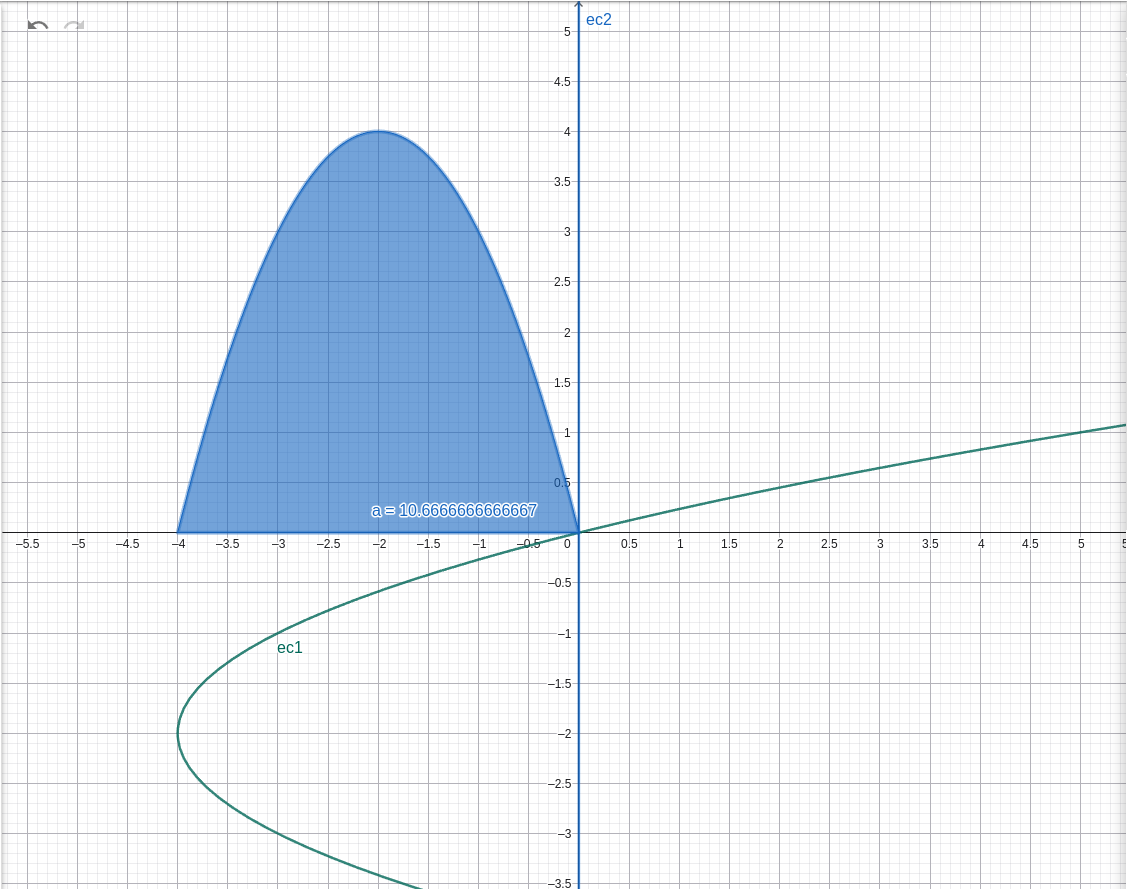
\includegraphics[width=0.5\textwidth]{Graficas/ejer19.png}
\end{center}
